\section{Mathematical Background: Category Theory}

The fundaments of ZX-Calculus are based on the mathematical model of Category-theory. A category is an abstract mathematical model which consists of a class of objects and a set of morphisms \cite{quanlong2023completness}. Objects represent the current \textit{state} of the calculation, whereas morphisms act like logic gates, which map between those objects. In particular, a ZX-diagram is represented by strict compact closed symmetric monoidal category \cite{emmanueljeandel2020zx}. Which has (among other things) the following properties:

Given such a category $\mathcal{C}$ with objects $\{A, B, C, D\}$ and morphisms $\{f: A \rightarrow B, g: B \rightarrow C, h: C \rightarrow D\}$, there exists a notion of composition \label{sequential-composition}. Therefore, we can compose morphisms that are applied sequentially to get new morphisms. We can, for example, combine $f$ and $g$ to get the morphism $g \circ f: A \rightarrow C$. The composition operator is associative. Thus the following statement holds $(h \circ g) \circ f = h \circ (g \circ f)$. An identity morphism $id_A: A \rightarrow A$ exists for each object $A$. This identity morphism is neutral concerning composition, meaning that $f \circ id_A = f = id_B \circ f$.

There also exists a Bifunctor $\otimes:\mathcal{C}\times\mathcal{C}\rightarrow\mathcal{C}$ which is used to combine multiple \textit{parallel} morphisms into a single morphism \label{parallel-composition}. In our example, we can combine $f$ and $g$ to get a new morphism $f \otimes g: A \otimes B \rightarrow C \otimes D$. This Bifunctor is also associative, meaning that $(f \otimes g) \otimes h = f \otimes (g \otimes h)$ always holds. Furthermore, there exists a unit object $I$ which acts as a neutral element concerning the Bifunctor, meaning that $f \otimes I = f = I \otimes f$ for each morphism $f$.

The category also provides a natural isomorphism $\sigma_{A, B}: A \otimes B \rightarrow B \otimes A$ for each pair of objects $A$ and $B$. This means that swapping the order of objects is always possible.

Finally, there also exists a notion of dual objects. Given an object $A$, there exists a dual object $A^*$. By using the special morphisms $\eta_A: I \rightarrow A \otimes A^*$ and $\epsilon_A: A^* \otimes A \rightarrow I$, we can introduce a notion of \textit{entanglement}-morphisms. These unique morphisms are called \textit{CAP} and \textit{CUP}, respectively. We will see later that these morphisms can be used to introduce entangled quantum states such as the Bell pairs.

\subsection{Quantum Circuits based on Category Theory}

Using the mathematical model of category theory, we can now define a quantum circuit based purely on objects and morphisms. We will restrict our category to the category of finite dimensional Hilbert spaces and linear maps to achieve a concrete model. Particularly, this means that the class of the objects in our category are finite-dimensional Hilbert spaces, and the morphisms are linear maps between those Hilbert spaces. This category is denoted as $\mathbf{FDHilb}$. Furthermore, we define the sequential composition of morphisms as the matrix multiplication of the underlying linear maps. The Bifunctor $\otimes$ is defined as the Kronecker product respectively.

\begin{figure}[h]
    \centering
    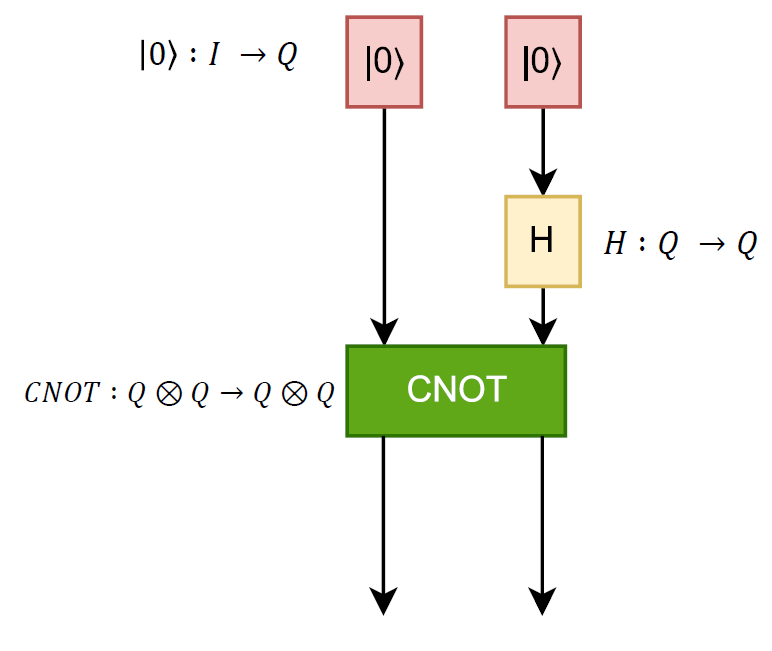
\includegraphics[height=5cm]{images/category-circuit.png}
    \caption{Circuit for creating Bell pairs}
    \label{fig:bell_circuit}
\end{figure}

Using this model, we can now define an actual circuit: We will look at the entanglement circuit shown in figure \ref{fig:bell_circuit}. This circuit produces entangled qubit pairs. Note that the visual representation looks very similar to the classical gate-based circuit. The only difference is that we translate it to use the morphisms of our category instead of the gates.


The circuit shown in figure \ref{fig:bell_circuit} consists of three morphisms.

\begin{itemize}
    \item $|0\rangle$ is defined as the morphism $I\rightarrow Q$ which initializes a qubit to the state $|0\rangle$.
    \item $H$ is a morphism of the form $Q\rightarrow Q$. It is a linear map between two qubits, acting as a single qubit Hadamard gate.
    \item $CNOT$ is the controlled-not gate, analogously to the classical \textbf{CNOT} gate, it represents a linear map from two qubits to two qubits. It is a morphism of the form $Q\otimes Q \rightarrow Q \otimes Q$.
\end{itemize}

At the moment, we are only able to define the circuit abstractly. As we only represented the circuit using the abstract morphisms from above. In the next section, we will describe the objects and morphisms used in the category, thereby introducing the basic building blocks of ZX-Calculus.

